\documentclass[12pt]{article}
%%%%%%%%%%%%%%%%%%%%%
% Header material
%%%%%%%%%%%%%%%%%%%%%

%%%%%%%%%%%%%%%%%%%%%
%  Includes first
%%%%%%%%%%%%%%%%%%%%%
%\usepackage{amsfonts}
%\usepackage{epsf}
\usepackage{placeins}
\usepackage[papersize={8.5in,11in}]{geometry}
\usepackage[pdftex]{graphicx}
\DeclareGraphicsExtensions{.pdf,.png,.jpg}
%\usepackage{draftwatermark}
\usepackage{amsmath}
\usepackage{amsthm}
\usepackage{amssymb}
%\usepackage{txfonts}
\usepackage{textcomp}
%\usepackage{amsthm}
%\usepackage{array}
\usepackage[all]{xy}
\usepackage{fancyhdr}
\usepackage{hyperref}
\usepackage{verbatim}
\usepackage{algorithm}
\usepackage{algorithmic}
\usepackage{color}
\usepackage[usenames,dvipsnames,svgnames,table]{xcolor}
\usepackage{rotating}
\usepackage{wrapfig}
\usepackage{tikz}
\usetikzlibrary{shapes.geometric, arrows}
\usepackage{framed}
\usepackage{multicol}
\usepackage{physics}

\usepackage[utf8]{inputenc}

%%%%%%%%%%%%%%%%%%%%
%  Setup listing environment
%%%%%%%%%%%%%%%%%%%%
\usepackage{listings}
\lstset{language=python,frame=ltrb,framesep=5pt,basicstyle=\small,
 keywordstyle=\ttfamily\color{DarkRed},
%morecomment=[n][\textbf]{In\ [}{]\:},
%morecomment=[n][\textbf]{Out\ [}{]\:},
morecomment=[s][\color{blue}]{In\ [}{]\:},
morecomment=[s][\color{red}]{Out[}{]\:},
identifierstyle=\ttfamily\color{DarkBlue}\bfseries,
commentstyle=\color{OliveGreen},
stringstyle=\ttfamily,
showstringspaces=false,tabsize = 3,
numbers = left}
\usepackage[framemethod=TikZ]{mdframed}
%\usepackage{framed}

\lstdefinelanguage{shell} {
commentstyle = \color{black},
keywordstyle = \color{black},
stringstyle = \color{black},
identifierstyle = \color{black},
morecomment=[s][\color{blue}]{In\ [}{]\:},
morecomment=[s][\color{red}]{Out[}{]\:},
 }

%\definecolor{shadecolor}{gray}{0.9}
\definecolor{shadecolor}{rgb}{0.93,0.95,1.0}


%%%%%%%%%%%%%%%
%  Setup the title region
%%%%%%%%%%%%%%%
\newmdenv [
outerlinewidth = 2,
linecolor = DarkBlue,
roundcorner = 8pt,
leftmargin = 0,
rightmargin = 0,
backgroundcolor = blue!7,
outerlinecolor = blue!70!black,
innertopmargin = \topskip,
splittopskip = \topskip
] {mdtitle}


%%%%%%%%%%%%%
% A few commands
%%%%%%%%%%%%%
\def      \RR             {{\mathbb R}} 
\def      \DS            {\displaystyle} 

%\renewcommand\baselinestretch{1.3}
%% The following block is for narrow margins:
\setlength{\topmargin}{-0.9in}
\setlength{\textheight}{9.50in}
\setlength{\oddsidemargin}{-0.375in}
\setlength{\evensidemargin}{-0.375in}
\setlength{\textwidth}{7.25in}
%% end page descript.
\pagestyle{empty}

\graphicspath{{Resources/}}
\renewcommand{\thesection}{}
\renewcommand{\thesubsection}{}
\hypersetup{
    colorlinks=true,
    linktoc=all,
    citecolor=purple,
    filecolor=green,
    linkcolor=red,
    urlcolor=blue
}

%\makeatletter
%\newcommand{\thickhline}{%
%    \noalign {\ifnum 0=`}\fi \hrule height 1pt
%    \futurelet \reserved@a \@xhline
%}
%\newcolumntype{"}{@{\hskip\tabcolsep\vrule width 1pt\hskip\tabcolsep}}
%\makeatother

\renewcommand{\descriptionlabel}[1]{%
  \hspace\labelsep \upshape\bfseries #1:%
}

%%%%%%%%%%%%%%%%%%%%%%%%%%%
%% Document starts here
%%%%%%%%%%%%%%%%%%%%%%%%%%%

\begin{document}

%%%%%%%%%%%%
% Title
%%%%%%%%%%%%

%\begin{mdtitle}
%\begin{center}
%\begin{Large}
%Notes  \hfill  \scalebox{1.1}{Example Qubit States} \hfill Fall 2016 \\[2mm]
%Quantum Computing \hfill Scott Carda
%\end{Large}
%\end{center}
%\end{mdtitle}
%\vspace*{10mm}

\title{Ternary Emulation Manual}
\date{}
\author{Scott Carda}

\maketitle
\newpage

%%%%%%%%%%%%%%%%%%%%%%%%
%% Table of Contents 
%%%%%%%%%%%%%%%%%%%%%%%%

\tableofcontents
\newpage

%%%%%%%%%%%%
%% Body 
%%%%%%%%%%%%

\section{Introduction} \label{sec:Intro}

This manual describes the Emu Emulator, an emulation of a ternary logic machine. This emulator
exists as a python package and can be implemented in any python3 script. The basics of ternary
logic are described as well. 

\section{Ternary Logic} \label{sec:Logic}

While the base unit of binary computers is a bit, having two states, the base unit of ternary
computers is a trit, having three states. These states are represented in two ways: as the
numbers 0, 1, and 2, and and the truth values False, Neutral, and True, or F, N, and T,
respectively. The mapping between these two representations is 0 = F, 1 = N, and 2 = T.

\subsection{Representation}

Trits can be agglomerated into larger units called trytes, a tryte containing nine trits,
having $3^{9}$ states. This is the ternary complement to the binary byte. Because this is a
large number of bits, it is advantageous to use a more compact way of representing trytes rather
than spelling out the value of each trit. One way of accomplishing this is to interpret the
series of trits as digits of a number represented in the number base 3, and convert the number
to base 10. In this way, groups of trits can represent large numbers. This conversion, while
human readable, is too computationally intensive and inefficient to be used to significant degree
internally in the emulator. We will use the heptavigesimal numbering system, or hept for short,
which is base 27. Because the hept is base 27, which is a power of 3, the representation will map
directly to the values of the trits, unlike base 10. A single character in the hept system will
represent all 27 possible states of a group of three trits, so we will need three hept characters
to represent one tryte. The characters we will use for our implementation of the hept system will
start with the ampersat, or the “@” symbol, representing the zero state. Then states 1 through 26,
those being the base 10 conversions of the numbers acquired from interpreting the trits as base 3
numbers, will be represented by the letters A-Z of the alphabet, respectively.

\subsection{Logic Gates}

The three-valued nature of the trits makes them incompatible with the traditional binary logic
gates. A new set of logic gates must be used to construct logic on a ternary machine. We will be
using truth tables to represent the logic of an individual gate. For single input gates, the left
column represents the single trit input into the gate, and the right column represents the single
trit output. For two input gates, the leftmost column acts as an axis and represents the first of
the two trit inputs. The topmost row acts as an axis and represents the second of the two trit
inputs. The rest of the table represents the output values of the single output trit. The following
are several logic gates that are defined:

\begin{figure}[h]
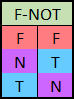
\includegraphics[scale=1]{Resources/FNOT.PNG}
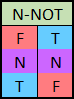
\includegraphics[scale=1]{Resources/NNOT.PNG}
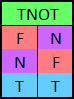
\includegraphics[scale=1]{Resources/TNOT.PNG}
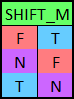
\includegraphics[scale=1]{Resources/SHIFT_M.PNG}
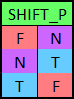
\includegraphics[scale=1]{Resources/SHIFT_P.PNG}
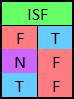
\includegraphics[scale=1]{Resources/ISF.PNG}
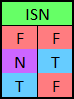
\includegraphics[scale=1]{Resources/ISN.PNG}
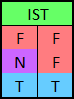
\includegraphics[scale=1]{Resources/IST.PNG}
\end{figure}

\begin{figure}[h]
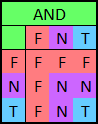
\includegraphics[scale=1]{Resources/AND.PNG}
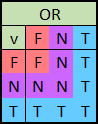
\includegraphics[scale=1]{Resources/OR.PNG}
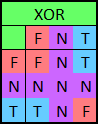
\includegraphics[scale=1]{Resources/XOR.PNG}
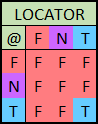
\includegraphics[scale=1]{Resources/LOCATOR.PNG}
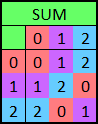
\includegraphics[scale=1]{Resources/SUM.PNG}
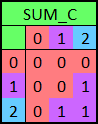
\includegraphics[scale=1]{Resources/SUM_C.PNG}
\end{figure}

\section{The Emu Emulator} \label{sec:Emu}

The Emu Emulator is an emulator for a ternary computing system. It uses a 27-trit instruction
set, and a word in this machine is 27 trits, or three trytes. The 9 programmable index registers,
as well as the program counter, or PC, are all single word registers. The current program status
register, or CPSR, is a register with three trits flags in it that keep track of the qualities of
the results of certain operations, which can be used to dictate the program flow. Programs are
stored in RAM as a series of instructions and data. RAM is a 27-trit address space that is
word-addressable.

The Emu emulator can be used in a python script by importing the Emulator package. Create an Emu
object, then use the member function “read\_object”, passing the path to an object file, prepared
ahead of time, as a string. This will read the program, represented by the object file, into the
RAM of the Emu object. Finally, call the member function “start” to have the program executed by
the Emu Emulator object.

\section{Instruction Format} \label{sec:Format}
               
\begin{figure}[h!]
    \centering
    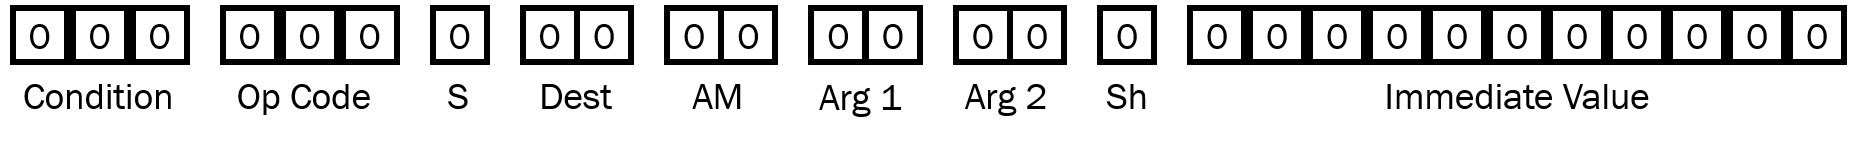
\includegraphics[width=\linewidth]{Resources/Instruciton_Format.png}
    \caption
    {
        27-trit Instruciton Format
    } \label{fig:Instruction Format}
\end{figure}

\begin{description}
\item[Condition] The 3-trit condition code the machine uses to determine whether the instruction is executed.
\item[Op Code] The 3-trit code that indicates which operation is performed with this instruction.
\item[S] The instruction's flag mode. The jump operation has unique behavior associated with this.
\item[Dest] The 2-trit indicator for the destination register.
\item[AM] The instruction's 2-trit address mode.
\item[Arg 1] The 2-trit indicator for the register to be used as the first argument to the operation.
\item[Arg 2] The 2-trit indicator for the register to be used as the second argument to the operation.
\item[Sh] The instruction's shift mode. Indicates which shift operation is performed on Arg 2.
\item[Immediate Value] This 11-trit field is reserved for embedding numerical values in the instruction.
\end{description}
    
\section{Conditions} \label{sec:Conditions}

The Current Program Status Register or CPSR is a special 3-trit register that keeps track of several
flags. There are three flag, one associated with each of the three trits in the register. The most
significant trit is the \textbf{S} flag, which indicates the sign of the result of an operation.
\hyperref[tab:S Flag Values]{Table \ref{tab:S Flag Values}} shows the meaning of the values for the
\textbf{S} flag. The middle of the three trits is the \textbf{C} flag, which contains the value of
any unsigned overflow resulting from an operation. The least significant trit is the \textbf{V} flag,
which contains the value of any signed overflow resulting from an operation.

\begin{table}[h!]
    \centering
    %\caption{\textbf{S} Flag Values}
    \caption{}
    \label{tab:S Flag Values}
    \begin{tabular}{|c|l|} 
        \hline
        %\textbf{S} & Meaning \\ [0.5ex] \hline
        \textbf{S} Flag & Meaning \\ \hline
        0 & Result was Positive \\ \hline
        1 & Result was Zero \\ \hline
        %2 & Result was Negative \\ [1ex] \hline
        2 & Result was Negative \\ \hline
    \end{tabular}
\end{table}

Instruction are conditionally executed based on the values of these flag. Common conditions have been
abstracted from these flag and made available to the system. Each condition is assigned a 3-trit code
for use in the most significant field of an instruction. If the condition is false, the rest of the
instruction is ignored, and the machine will move on to the next instruction in its RAM without executing
the encoded operation. The conditions available to the system are found in
\hyperref[tab:Conditions]{Table \ref{tab:Conditions}}. As this is a 3-trit code, each of these condition
codes can be represented as a single heptavigesimal character, which are found in parentheses in the
first column of the table.

\begin{table}[h!]
    \centering
    \caption{}
    \label{tab:Conditions}
    \begin{tabular}{|c|l|c|} 
        \hline
        \textbf{Condition Code} & Meaning & Flags \\ \hline
        
        000 (@) & Always & Always \\ \hline
        001 (A) & Equal & \textbf{S} = 1 \\ \hline
        002 (B) & Carry Clear & \textbf{C} = 0 \\ \hline
        010 (C) & Negative & \textbf{S} = 2 \\ \hline
        011 (D) & Overflow Clear & \textbf{V} = 0 \\ \hline
        012 (E) & Unsigned Lower/Equal & \textbf{C} = 0 \textbf{OR} \textbf{S} = 1 \\ \hline
        020 (F) & Less Than & IS\_T(\textbf{S}) = IS\_F(\textbf{V}) \\ \hline
        021 (G) & Less Than or Equal To & \textbf{S} = 1 \textbf{OR} IS\_T(\textbf{S}) = IS\_F(\textbf{V}) \\ \hline
    
        022-200 (H-R) & \textit{bad condition code} & \textit{bad condition code} \\ \hline
    
        201 (S) & Greater Than & \textbf{S} $\neq$ 1 \textbf{AND} IS\_T(\textbf{S}) $\neq$ IS\_F(\textbf{V}) \\ \hline
        202 (T) & Greater Than or Equal To & IS\_T(\textbf{S}) $\neq$ IS\_F(\textbf{V}) \\ \hline
        210 (U) & Unsigned Higher & \textbf{C} $\neq$ 0 \textbf{AND} \textbf{S} $\neq$ 1 \\ \hline
        211 (V) & Overflow Set & \textbf{V} $\neq$ 0 \\ \hline
        212 (W) & Positive & \textbf{S} $\neq$ 2 \\ \hline
        220 (X) & Carry Set & \textbf{C} $\neq$ 0 \\ \hline
        221 (Y) & Not Equal & \textbf{S} $\neq$ 1 \\ \hline
        222 (Z) & Never & Never \\ \hline
    \end{tabular}
\end{table}

\section{Operations} \label{sec:Operations}

The emulator supports 24 operations, which are listed in \hyperref[tab:Opcodes]{Table \ref{tab:Opcodes}} along
with their associated opcodes.

\begin{table}[h!]
    \centering
    \caption{}
    \label{tab:Opcodes}
    \begin{tabular}{|c|l|c|} 
        \hline
        \textbf{Operation Code} & Operation \\ \hline

        000 (@) & HALT \\ \hline
        001 (A) & NO\_OP \\ \hline
        002 (B) & CLEAR \\ \hline

        010 (C) & LOAD \\ \hline
        011 (D) & STORE \\ \hline
        012 (E) & EXCHANGE \\ \hline

        020 (F) & ADD \\ \hline
        021 (G) & SUB \\ \hline
        022 (H) & MOVE \\ \hline

        100 (I) & AND \\ \hline
        101 (J) & OR \\ \hline
        102 (K) & XOR \\ \hline

        110 (L) & FNOT \\ \hline
        111 (M) & NNOT \\ \hline
        112 (N) & TNOT \\ \hline

        120 (O) & ISF \\ \hline
        121 (P) & ISN \\ \hline
        122 (Q) & IST \\ \hline

        200 (R) & LSR \\ \hline
        201 (S) & ASR \\ \hline
        202 (T) & LSL \\ \hline

        210 (U) & SHIFT\_M \\ \hline
        211 (V) & SHIFT\_P \\ \hline
        212 (W) & \textit{bad operation code} \\ \hline

        220 (X) & JUMP \\ \hline
        221 (Y) & \textit{bad operation code} \\ \hline
        222 (Z) & \textit{bad operation code} \\ \hline
    \end{tabular}
\end{table}

\begin{description}
\item[HALT] Raises a HALT exception, causing the current program to stop executing.
This should be considered the proper way for a program to terminate.
\item[NO\_OP] Will not perform any operation, other than to move the current program counter to the
next instruction.
\item[CLEAR] Sets the word of memory at the specified address to all zeros, clearing the memory location.
\item[LOAD] Loads the word of memory at the specified address into the destination register.
\item[STORE] Stores the contents of the destination register into memory at the specified address.
The register specified by the \textbf{Dest} field is actually used as the data source in this instruction.
\item[EXCHANGE] Loads the word of memory at the specified address into the destination register,
while storing the original value of the destination register at the specified address in memory,
effectively swapping the two values.
\item[ADD] Adds together the values in the registers specified by \textbf{Arg1} and \textbf{Arg2},
storing the result in the destination register.
\item[SUB] Subtracts the value in the register specified by \textbf{Arg2} from the value in the register
specified by \textbf{Arg2}, storing the result in the destination register.
\item[MOVE] Copies the value specified into the destination register.
\item[AND] Tritwise AND the values in the registers specified by \textbf{Arg1} and \textbf{Arg2},
storing the result in the destination register.
\item[OR] Tritwise OR the values in the registers specified by \textbf{Arg1} and \textbf{Arg2},
storing the result in the destination register.
\item[XOR] Tritwise XOR the values in the registers specified by \textbf{Arg1} and \textbf{Arg2},
storing the result in the destination register.
\item[FNOT] Tritwise FNOT the value in the register specified by \textbf{Arg2}, ignoring \textbf{Arg1}.
\item[NNOT] Tritwise NNOT the value in the register specified by \textbf{Arg2}, ignoring \textbf{Arg1}.
\item[TNOT] Tritwise TNOT the value in the register specified by \textbf{Arg2}, ignoring \textbf{Arg1}.
\item[ISF] Tritwise ISF the value in the register specified by \textbf{Arg2}, ignoring \textbf{Arg1}.
\item[ISN] Tritwise ISN the value in the register specified by \textbf{Arg2}, ignoring \textbf{Arg1}.
\item[IST] Tritwise IST the value in the register specified by \textbf{Arg2}, ignoring \textbf{Arg1}.
\item[LSR] Shifts all the trit values in the register specified by \textbf{Arg1} to the right by
the specified number of trits, resulting in a division of the number by a power of three. The result is
stored in the destination register. The trit value shifted into the most significant trit will be zero.
\item[ASR] Shifts all the trit values in the register specified by \textbf{Arg1} to the right by
the specified number of trits, resulting in a division of the number by a power of three. The result is
stored in the destination register. The trit value shifted into the most significant trit will be two
if the original value was negative, or zero otherwise, preserving the sign of the value. 
\item[LSL] Shifts all the trit values in the register specified by \textbf{Arg1} to the left by
the specified number of trits, resulting in a multiplication of the number by a power of three. The
result is stored in the destination register. The trit value shifted into the most significant trit will
be zero.
\item[SHIFT\_M] Tritwise SHIFT\_M the value in the register specified by \textbf{Arg2}, ignoring \textbf{Arg1}.
\item[SHIFT\_P] Tritwise SHIFT\_P the value in the register specified by \textbf{Arg2}, ignoring \textbf{Arg1}.
\item[JUMP] Puts the value of the register specified by \textbf{Arg2} into the PC register, causing the
program execution to jump to that address in RAM. This operation has special logic associated with the
flag mode of the instruction.
\end{description}

\section{Flag Mode} \label{sec:Flag Mode}

This is a single-trit field in the instruction that denotes the flag mode for the instruction. There are
three flag modes that can be used, the value this field takes for each mode is outlined in
\hyperref[tab:S Field Values]{Table \ref{tab:S Field Values}}. 'No-Set' mode will prevent the instruction from
affecting the CPSR register flags. 'Set' mode will allow for the instruction to set the flags in the CPSR
register. 'Exclusive-Set' mode will allow for the instruction to set the flags in the CPSR register, while
throwing out the usual result of the instruction, instead of storing it to the destination register.

\begin{table}[h!]
    \centering
    %\caption{\textbf{S} Flag Values}
    \caption{}
    \label{tab:S Field Values}
    \begin{tabular}{|c|l|}
        \hline
        \textbf{S} Field & Flag Mode \\ \hline
        0 & Result was No-Set \\ \hline
        1 & Result was Set \\ \hline
        2 & Result was Exclusive-Set \\ \hline
    \end{tabular}
\end{table}

The jump instruction has speacial logic associated with this field. As the jump instruction cannot
affect the CPSR flags, the regular flag modes are not applicable. Instead this value is used to
determine how to handle capturing the current value in the PC register. If the value of this field
is 0, the current location in code, before the jump, is not recorded, and Destination field is
ignored. If the value is 1, the current location in code, before the jump, is stored in the register
denoted in the Destination field. This is done to make it easier to implement functions by capturing
where the function will return to. If the value of the field is 2, the jump will not affect the PC
register, resulting in no jump in code, but will store the current value in the PC register in
the register denoted in the Destination field.

\section{Address Mode} \label{sec:Address Mode}

There are 8 address modes, which are listed in table
\hyperref[tab:Address Modes]{Table \ref{tab:Address Modes}}. The first 3 address modes, 00 through 02,
are used by non-addressing operations, such as add or sub. The last 5 address modes are used by
addressing instructions, such as ldr and str. The address mode dictates the value of the
second argument to the operation, or the only argument to the operation for operations that
only have one argument. For addressing operations, this value must be an address.

\begin{table}[h!]
    \centering
    \caption{}
    \label{tab:Address Modes}
    \begin{tabular}{|c|l|}
        \hline
        \textbf{AM} Field & Address Mode \\ \hline
        00 & Immediate \\ \hline
        01 & Register Direct \\ \hline
        02 & Register Direct Scaled \\ \hline
        10 & \textit{bad address mode} \\ \hline
        11 & Addressed \\ \hline
        12 & Register Indirect \\ \hline
        20 & Immediate Offset \\ \hline
        21 & Direct Offset \\ \hline
        22 & Scaled Offset \\ \hline
    \end{tabular}
\end{table}

\begin{description}
\item[Immediate] The value of the immediate field is used as the argument.
\item[Register Direct] The value of the register indicated by Arg 2 is used as the argument.
\item[Register Direct Scaled] The value of the register indicated by Arg 2 undergoes a shift
operation, indicated by the instruction's shift mode, whose magnitude is the value of the
immediate field. The result is used as the argument.
\item[Addressed] The value of the immediate field is the address used as the argument.
\item[Register Indirect] The address found in the register indicated by Arg 1 is used as the
argument.
\item[Immediate Offset] The sum of the address found in the register indicated by Arg 1 and
the value of the immediate field is the address used as the argument.
\item[Direct Offset] The sum of the address found in the register indicated by Arg 1 and the
value of the register indicated by Arg 2 is the address used as the argument.
\item[Scaled Offset] The value of the register indicated by Arg 2 undergoes a shift operation,
indicated by the instruction's shift mode, whose magnitude is the value of the immediate field.
The result is added to the address found in the register indicated by Arg 1, resulting in the
address used as the argument.
\end{description}

\section{Shift Mode} \label{sec:Shift Mode}

This is a single-trit field in the instruction that denotes the flag mode for the instruction.
There are three flag modes that can be used, the value this field takes for each mode is
outlined in \hyperref[tab:Shift Modes]{Table \ref{tab:Shift Modes}}. There are two address
modes which perform a scaling operation, Register Direct Scaled and Scaled Offset. In these
address modes the value of the register indicated by Arg 2 undergoes a shift operation whose
magnitude is the value of the immediate field. The shift mode indicates which shift operation
is performed during these instructions.

\begin{table}[h!]
    \centering
    \caption{}
    \label{tab:Shift Modes}
    \begin{tabular}{|c|l|}
        \hline
        \textbf{Sh} Field & Shift Mode \\ \hline
        0 & Logical Shift Right \\ \hline
        1 & Arithmetic Shift Right \\ \hline
        2 & Logical Shift Left \\ \hline
    \end{tabular}
\end{table}

\section{Immediate Value} \label{sec:Immediate Value}

The last 11 trits of an instruction represent a numerical value embedded in the
instruction. This field is further subdivided into a rotation field, which is the
first 2 trits, and the value field, which is the remaining 9 trits. The number that
the immediate represents is calculated by treating the value field as the least
significant 9 trits in a 27-trit number. That number is then rotated to the right
by 3 times the number specified in the rotation field. The resulting number may be 
interpreted as a signed or unsigned number depending on its use.

%\include{Sections/Bloch_Sphere}

%\include{Sections/Mathy}

%\include{Sections/Transformation_Definitions}

%\include{Sections/Examples}

\end{document}
